% =====================================================================
% Cross-Family Symbolic Verification for Contamination-Robust LLM Math
%
% Guide / model introduction used for structure and pacing:
%   Zhou, Staats, Li, Szegedy, Weinberger, Feng. (2024).
%   "Don't Trust: Verify -- Grounding LLM Quantitative Reasoning with
%   Autoformalization." ICLR.
%   PDF: https://arxiv.org/pdf/2403.18120
%
% A second model used for selective-prediction framing:
%   Kuhn, Gal, Farquhar. (2023). "Semantic Uncertainty: Linguistic
%   Invariances for Uncertainty Estimation in Natural Language
%   Generation." ICLR.  PDF: https://arxiv.org/pdf/2302.09664
% =====================================================================
\documentclass[11pt]{article}

\usepackage[utf8]{inputenc}
\usepackage[T1]{fontenc}
\usepackage[margin=1in]{geometry}
\usepackage[hidelinks]{hyperref}
\hypersetup{
  colorlinks=true,
  linkcolor=black,
  citecolor=black,
  urlcolor=black,
  filecolor=black,
  menucolor=black,
  anchorcolor=black,
  pdfborder={0 0 0},
}
\usepackage{url}
\usepackage{booktabs}
\usepackage{amsfonts}
\usepackage{amsmath}
\usepackage{amssymb}
\usepackage{graphicx}
\usepackage{xcolor}
\usepackage{microtype}
\usepackage[numbers,round,sort&compress]{natbib}
\usepackage{multirow}
\usepackage{caption}
\usepackage{enumitem}
\usepackage{setspace}
\usepackage{titlesec}
\usepackage{tikz}
\usetikzlibrary{arrows.meta,positioning,calc,shapes}
\usepackage{listings}
\lstdefinestyle{xsgrv}{
  basicstyle=\ttfamily\footnotesize\color{black},
  keywordstyle=\color{black},
  commentstyle=\color{black},
  stringstyle=\color{black},
  identifierstyle=\color{black},
  numberstyle=\color{black},
  numbers=none,
  frame=single,
  framesep=4pt,
  rulecolor=\color{black},
  breaklines=true,
  showstringspaces=false,
  xleftmargin=0pt,
  language=Python,
}

\setlength{\parindent}{18pt}
\setlength{\parskip}{3pt}
\onehalfspacing
\titleformat{\section}{\large\bfseries}{\thesection.}{0.5em}{}
\titleformat{\subsection}{\normalsize\bfseries}{\thesubsection}{0.5em}{}

\renewcommand{\bibsection}{\section*{References}}
\setlength{\bibsep}{2pt plus 0.3ex}

\title{\bfseries Cross-Family Symbolic Verification for Contamination-Robust Mathematical Reasoning by Large Language Models}
\author{
Aayan Alwani$^{1}$, Ashley Laughney$^{2}$ \\[2pt]
\small $^{1}$Great Neck South High School, Lake Success, NY, USA \\
\small $^{2}$Englander Institute for Precision Medicine, Weill Cornell Medicine, New York, NY, USA
}
\date{}

\begin{document}
\maketitle

% =====================================================================
\section*{Summary}
% =====================================================================

Large language models (LLMs) increasingly produce mathematical reasoning that is reused in scientific computing, education, and decision support, yet the field still lacks a reliable way to know when an LLM's answer should be trusted \citep{kuhn2023semantic, farquhar2024nature}. Same-model self-verification --- in which the model writes a Python check for its own work --- fails on the Mathematical Aptitude Test of Heuristics (MATH) benchmark because errors in the reasoning leak into the assertions that are supposed to catch them \citep{huang2024selfcorrect, tyen2024llm, stechly2024selfverify}. Existing benchmark-based confidence signals are further inflated because the most common evaluation set, MATH-500, is reproduced verbatim 54.6\% of the time by Qwen2.5-Math-7B, indicating training-data contamination \citep{wu2025contam}. The present study measures both failure modes and proposes a remedy called X-SGRV (cross-family symbolic verification). A different LLM, drawn from a different model family than the one solving the problem, reads only the problem statement and emits a short Python/SymPy function $\texttt{verify(answer)}$ that is run inside a sandboxed subprocess against the candidate answer. Two deployment-safe additions further harden the signal: an adversarial filter that perturbs the candidate (never the gold) to expose verifiers that accept clearly wrong values, and consensus across two or more cross-family extractors. On the full MATH-500 benchmark ($n{=}498$), cross-extractor consensus accepts 171 of 498 candidates and is correct on all 171 (Clopper-Pearson 95\% confidence interval 0.979--1.000), fulfilling a pre-registered branch committed before the scale-up.\footnote{Pre-registration document: \texttt{PRE\_COMMIT\_n500.md} in the project repository, timestamped before the scale-up was launched.} Five frontier extractors --- one from each major laboratory (Meta, DeepSeek, OpenAI, Anthropic, Alibaba) --- agree on 69 problems and are correct on all 69. On contamination-clean competition benchmarks (American Invitational Mathematics Examination 2025 and a 125-problem combo of Harvard-MIT Math Tournament, Brown Math Olympiad, Stanford Math Tournament, and APEX 2025), every prior agreement-based selective-prediction signal collapses, while X-SGRV correctly abstains on the structurally unverifiable majority and remains accurate on the small accepted subset. These results show that grounding the verifier in the problem specification, drawing it from a different model family than the solver, and demanding consensus together produce a deployment-safe abstention signal for LLM mathematical reasoning that does not require gold labels at deployment time.

% =====================================================================
\section{Introduction}
% =====================================================================

\noindent
{\small\textit{Model introduction used as a writing guide:} Zhou et al.\ (2024) ``Don't Trust: Verify -- Grounding LLM Quantitative Reasoning with Autoformalization,'' ICLR. PDF: \url{https://arxiv.org/pdf/2403.18120}. A second guide for selective-prediction framing was Kuhn, Gal, and Farquhar (2023), ``Semantic Uncertainty,'' ICLR, PDF: \url{https://arxiv.org/pdf/2302.09664}. The structural choices in the introduction below --- opening with the broad capability and societal stake, narrowing to the verification problem, surveying prior diagnoses, and ending with a numbered aim list --- mirror the inverted-pyramid order used in those works.\par}
\medskip

Large language models have become a default tool for solving mathematical word problems and competition tasks, with chain-of-thought prompting raising arithmetic accuracy on grade-school benchmarks from below 20\% to above 80\% within two years of its introduction \citep{wei2022cot, cobbe2021gsm8k}. Mathematical reasoning generated by these models is now used as training data for downstream educational tools, as a proxy benchmark for general reasoning capability, and as a step inside scientific-computing pipelines that include numerical analysis and symbolic mathematics \citep{hendrycks2021math, lightman2024prm}. Recent reasoning-specialized systems such as DeepSeek-R1 have further extended this capability to harder competition mathematics, suggesting that mathematical reasoning will continue to expand as a deployed capability rather than remain confined to research benchmarks \citep{deepseek2025r1, mathshepherd2024}. Because errors in mathematical answers can be silent and difficult to detect at scale, downstream applications need a way to flag, before deployment, which model outputs are trustworthy and which should be escalated to a human or a stronger system; this problem is known as selective prediction \citep{kuhn2023semantic, farquhar2024nature}. Without such a signal, errors propagate quickly into curated training corpora, automated tutoring, and scientific workflows that consume model outputs, and the cost of an undetected error rises with the centrality of the downstream pipeline that consumes the answer \citep{ste2024, processbench2024, reasoneval2024}.

The dominant prior approach to selective prediction on mathematical reasoning has been some form of self-verification, in which the model that produced the answer is also asked to check it \citep{huang2024selfcorrect, stechly2024selfverify}. Self-verification can take the form of asking the model to rate its own confidence \citep{xiong2024llmuncertainty}, generating multiple solutions and scoring agreement \citep{wang2023selfconsistency}, asking the model to translate its solution into Python or another verifier-friendly language and run it \citep{symcode2024, prove2024, mathcoder2024}, or training a separate model called a process reward model on step-level correctness labels \citep{lightman2024prm, mathshepherd2024, qwenprm2025}. The most recent process-reward-model variants combine generative chain-of-thought with code execution, scale test-time compute on the verification side, or use formal-verification labels in place of human annotations, all aiming to tighten the verifier signal without changing the underlying solver \citep{genprm2025, fover2025, prime2025}. Each of these strategies achieves competitive results on the widely used MATH-500 dataset, with reported precisions above 90\% on the highest-confidence tier \citep{qwenprm2025, skyworkprm2024, rstarmath2025}.

A growing body of evidence indicates that these reported gains do not transfer to harder, contamination-clean problems. Huang et al.\ (2024) showed that intrinsic self-correction degrades reasoning performance on the GSM8K dataset and other benchmarks \citep{huang2024selfcorrect}. Tyen et al.\ (2024) and Stechly et al.\ (2024) demonstrated that LLMs cannot reliably localize their own errors and that self-verification produces high false-positive rates \citep{tyen2024llm, stechly2024selfverify}. Kim et al.\ (2025) analyzed more than 350 LLMs and found that larger and more accurate models exhibit \emph{more} correlated errors, not fewer, suggesting that the failure mode is structural and not solvable by simply scaling up \citep{kim2025correlated}. Wu et al.\ (2025) directly measured benchmark contamination on MATH-500: when prompted with the first 60\% of each problem, Qwen2.5-Math-7B reproduces 54.6\% of the original answers verbatim, and the same solver's accuracy drops from 76.6\% to 10\% on problems released after its training cutoff \citep{wu2025contam}. The MathArena leaderboard, which auto-refreshes with newly released competitions, shows similar drops across multiple LLM families and is recommended as a contamination-clean alternative to MATH-500 \citep{matharena2025}. The MATH-Perturb benchmark applies hard perturbations to Level-5 MATH problems and reports a similar decline in solver accuracy, providing additional independent evidence that high MATH-500 accuracy is partly memorization-driven \citep{mathperturb2025}. High top-tier precision on MATH-500 therefore cannot be attributed to verification reliability without a contamination-clean control \citep{wu2025contam, matharena2025}.

A second line of work has tried to break the dependency between solver and verifier by autoformalizing the problem statement into a formal language. Zhou et al.\ (2024) introduced the Don't-Trust-Verify framework, in which an Isabelle theorem prover checks an autoformalized version of the problem \citep{dtv2024}. Hermes (2025) extends this idea to Lean 4 by interleaving natural language with formal proof scripts \citep{hermes2025}. These specification-grounded approaches address the correlated-error concern in principle but require a heavyweight formal-methods stack and human-curated formal libraries; reported coverage on competition-level problems remains below 20\% in most cases \citep{dtv2024, hermes2025}. The Open Proof Corpus and related evaluations have begun to characterize the quality of LLM-generated mathematical proofs, but conclude that the autoformalization pipeline still rejects the majority of competition problems before any verification can begin \citep{openproof2025}. Lighter-weight randomized property-based testing has been applied to LLM-generated code \citep{pgs2025, quickcheck2000} but has not been combined with cross-model independence on natural-language mathematical reasoning, and step-level error-detection benchmarks have shown that LLMs alone cannot localize their own mathematical errors at the precision required for downstream filtering \citep{cannotspot2025, processbench2024}.

A third line of work uses agreement-based or entropy-based signals. Self-consistency generates multiple samples and uses majority vote \citep{wang2023selfconsistency}, while semantic entropy clusters samples by meaning (using either a symbolic solver or a natural-language inference model) and treats low entropy as high confidence \citep{kuhn2023semantic, farquhar2024nature}. Both methods report area-under-receiver-operator-characteristic values above 0.7 on MATH-500, and a Nature-published extension uses bidirectional natural-language inference to detect hallucinations across question-answering benchmarks \citep{kuhn2023semantic, farquhar2024nature, wang2023selfconsistency}. Cheaper variants such as semantic-entropy probes have since been proposed to reduce the multi-sample cost of these methods \citep{seprobes2024}. The complementary $p(\textsc{True})$ baseline asks the model to evaluate its own answer as ``True'' or ``False'' and reads the log-probability of the first token as a continuous confidence score \citep{kadavath2022}. However, when the underlying solver is uniformly uncertain --- as on competition problems released after the training cutoff --- agreement-based signals lose discriminating power, and when the solver is uniformly and confidently wrong, entropy-based signals can become anti-reliable because the entailment classifier collapses textually similar wrong answers into a single confident-looking cluster \citep{wu2025contam, kuhn2023semantic, farquhar2024nature}.

A specification-grounded selective-prediction signal that (a) does not require formal-methods infrastructure, (b) does not depend on solver agreement, (c) preserves structural independence between solver and verifier, and (d) maintains non-trivial coverage on contamination-clean benchmarks does not currently exist in the literature. Constructing such a signal would close a recognized gap in deployment-safe LLM evaluation and would make selective prediction tractable for downstream applications that require contamination-robust trust signals \citep{kuhn2023semantic, ste2024, dtv2024}. The closest existing approach in spirit is the autoformalization pipeline of Don't-Trust-Verify, which checks an Isabelle translation of the problem rather than the model's solution, but its dependence on a curated formal library limits coverage and rules out integration with the lightweight Python tooling that production LLM deployments already use \citep{dtv2024, hermes2025}.

The present study had three aims. First, to measure same-model self-verification failure rates on MATH-500 stratified by problem difficulty and to establish that the failure rate scales monotonically with difficulty as predicted by the correlated-error-collapse hypothesis \citep{huang2024selfcorrect, tyen2024llm, stechly2024selfverify, kim2025correlated}. Second, to measure the collapse of standard agreement- and entropy-based signals on contamination-clean competition benchmarks (American Invitational Mathematics Examination 2025; a 125-problem CleanMath combo of Harvard-MIT Mathematics Tournament February 2025, Brown Math Olympiad 2025, Stanford Math Tournament 2025, and APEX 2025) and to compare these to MATH-500 baselines \citep{wu2025contam, matharena2025}. Third, to design and pre-register a cross-family symbolic verification method (X-SGRV) and evaluate it on the full MATH-500 benchmark and on contamination-clean competition benchmarks against state-of-the-art baselines, including Qwen2.5-Math-PRM-7B, Skywork-o1-Open-PRM, semantic entropy in both symbolic and natural-language inference variants, $p(\textsc{True})$, and self-consistency \citep{qwenprm2025, skyworkprm2024, kuhn2023semantic, farquhar2024nature, kadavath2022, wang2023selfconsistency}.

% =====================================================================
\section{Materials and Methods}
% =====================================================================

\subsection{Models}

All solver and extractor models were accessed through public application programming interfaces (APIs). The primary solver was Qwen2.5-7B-Instruct-Turbo, accessed through Together AI; the choice was constrained by the published contamination report on this family of models \citep{wu2025contam}. For supplementary solver-rotation experiments, DeepSeek-V3, DeepSeek-V3.1, DeepSeek-R1, and gpt-oss-120b were also used as solvers \citep{deepseek2025r1}. Five cross-family extractors were used: Meta's Llama-3.3-70B-Instruct-Turbo, DeepSeek-V3, OpenAI's gpt-oss-120b, Anthropic's Claude Sonnet 4.6, and Alibaba's Qwen3-Coder-480B; a sixth extractor, OpenAI's GPT-5-mini, was used for sensitivity analyses. A same-family ablation used Qwen2.5-7B-Instruct as the extractor (confounded by scale, 7B versus 70B+). Two open process reward models were run locally on a single A100-class graphics processing unit via Modal: Qwen2.5-Math-PRM-7B and Skywork-o1-Open-PRM-Qwen-2.5-7B \citep{qwenprm2025, skyworkprm2024}. Skywork-PRM was loaded at \texttt{torch\_dtype=torch.bfloat16} after a 32-bit float load was observed to silently exhaust GPU memory and return uniform 0.5 scores. The natural-language inference variant of semantic entropy used \texttt{microsoft/deberta-large-mnli} \citep{farquhar2024nature}.

\subsection{Benchmarks}

The MATH-500 benchmark \citep{hendrycks2021math, lightman2024prm} was used at two scales: a stratified subsample of $n=175$ problems (stratification by difficulty level L1 through L5) and the full $n=500$ benchmark, of which two problems failed to produce solver candidates within the timeout, leaving $n=498$ for analysis. The American Invitational Mathematics Examination 2025 (AIME 2025) was used in full, combining AIME I (released February 6, 2025) and AIME II (released February 12, 2025) for $n=30$ problems. A contamination-clean ``CleanMath'' combo was assembled from four mathematics competitions, all of which were released after the training cutoff of the Qwen2.5-Math-7B model documented in \citet{wu2025contam}: Harvard-MIT Mathematics Tournament February 2025 ($n=30$), Brown Math Olympiad 2025 ($n=30$), Stanford Math Tournament 2025 ($n=53$), and APEX 2025 ($n=12$), for a total of $n=125$ \citep{matharena2025}. A 100-problem subset of the hardest problems from Omni-MATH (difficulty 9.0--9.5 on a 10-point scale) was used as an out-of-distribution stress test \citep{omnimath2024}. For the proof-mode scope test, 100 random problems from PutnamBench were used \citep{amitayusht2024putnambench}.

\subsection{Solver pass}

For each problem, the solver was sampled greedily ($T=0$) once for the plurality-vote candidate and at $T=0.7$ ten times for entropy-based baselines. Generations were capped at 2048 tokens. The final answer was extracted from the last \texttt{\textbackslash boxed\{...\}} expression in the response; if no boxed expression was present, the last numeric or symbolic token of the last line was used as a fallback. Equivalence between predicted and gold answers was determined with SymPy \citep{meurer2017sympy} using a multi-strategy comparator (string match, normalized LaTeX, expanded difference, simplified difference, numerical evaluation), with a five-second timeout per comparison.

\subsection{Cross-family symbolic verification (X-SGRV)}

For each problem, the cross-family extractor was sent only the problem statement (never the solver's solution) and was prompted to emit a Python function $\texttt{verify(answer) -> bool}$ that re-derives the problem's constraints in SymPy plus standard library primitives ($\texttt{itertools}$, $\texttt{math}$, $\texttt{Fraction}$, $\texttt{Counter}$). The prompt explicitly forbade hard-coding the answer, required a strict abstention token (\texttt{UNVERIFIABLE}) when no bounded check was possible, and capped scripts at 60 lines. Extractor calls used $T=0.2$ and $\texttt{max\_tokens=2048}$. The full prompt is in the released code repository (file \texttt{src/xsgrv/extractor.py}).

The extracted script was executed in a sandboxed subprocess on the host laptop. The subprocess pre-imported $\texttt{sympy}$, $\texttt{math}$, $\texttt{itertools}$, $\texttt{fractions}$, and $\texttt{collections}$, and a $\texttt{SIGALRM}$-based timeout limited execution to 10 seconds per call. The verifier was tested against five candidate answers per problem: the gold answer, the solver's plurality-vote candidate, and four adversarial wrong candidates at gold $-1$, gold $+1$, gold $+7$, and a fixed alternative ($42$). A verifier was classified as ``working'' if it accepted the gold candidate and rejected all four adversarial wrong candidates.

\subsection{Deployment-time adversarial filter}

A second adversarial test ran independently of the gold answer and is therefore deployment-time-safe. The verifier was probed against four perturbations of the solver's candidate answer (candidate $-1$, candidate $+1$, candidate $+7$, candidate $\times 2$); for non-integer candidates, a deterministic fallback set $\{0, 1, -1, 42, 100\}$ was used after removing any value equal to the candidate. A verifier that accepted any probe was marked broken, and the pipeline abstained for that problem. The probe set was selected on a 30-problem held-out development split disjoint from the evaluation sets; the dev split was too small to discriminate between candidate probe sets (see Appendix) and the choice was kept on a-priori grounds.

\subsection{Cross-extractor consensus}

For each problem, two or more independent cross-family extractors were run. ``Strict consensus'' trusted a top-tier label only when every participating extractor produced a working verifier and every working verifier accepted the candidate. ``Loose consensus'' required at least one working verifier and every working verifier to accept. Two-extractor consensus (Llama $\cap$ DeepSeek) was used for the pre-registered MATH-500 scale-up; five-extractor consensus (Meta $\cap$ DeepSeek $\cap$ OpenAI gpt-oss $\cap$ Anthropic Claude $\cap$ Alibaba Qwen3-Coder) was used for the laboratory-agnostic test on MATH-175.

\subsection{Baselines}

Five baselines were implemented and run on cached solver samples to ensure matched-coverage comparisons with X-SGRV. (i) \emph{Verbalized confidence}: the solver was prompted to output a confidence between 0 and 1 after producing its answer \citep{xiong2024llmuncertainty}. (ii) \emph{Self-consistency}: the fraction of $k=4$ and $k=10$ samples voting for the modal answer using SymPy equivalence-class clustering \citep{wang2023selfconsistency}. (iii) \emph{Semantic entropy, symbolic}: 10 samples at $T=0.7$ clustered by SymPy equivalence; the negative log of the largest cluster size was used as the score \citep{kuhn2023semantic}. (iv) \emph{Semantic entropy, NLI}: the same 10 samples clustered by bidirectional entailment using DeBERTa-large-mnli \citep{farquhar2024nature}. (v) \emph{$p(\textsc{True})$}: the solver was asked ``Is this answer correct? True/False'' and the log-probability of the first token of the answer was read as a continuous score \citep{kadavath2022}. For PRMs, problem-level scores were obtained by taking the maximum aggregation across the 10 cached solver samples; all four common aggregations (min-step, mean-step, product-step, last-step) were reported \citep{qwenprm2025, skyworkprm2024}. PRM scoring protocols were validated against published ProcessBench numbers on a 48-problem subset \citep{processbench2024}; reproduction agreed within 5 F1.

\subsection{Statistical analysis}

Top-tier precision was reported as a proportion (top-tier accepts that were correct, divided by top-tier accepts) with Clopper-Pearson 95\% confidence intervals. Area-under-receiver-operator-characteristic values were reported with bootstrap 95\% confidence intervals from 1{,}000 resamples. Matched-binary comparisons between methods used McNemar's exact test. The 2$\times$2 ablation in the Results section used Fisher's exact test. Coverage was computed as the size of the top tier divided by the benchmark size.

\subsection{Pre-registration}

A pre-registration document, \texttt{PRE\_COMMIT\_n500.md}, was committed to the project repository with a timestamp before the $n=500$ scale-up was launched. The pre-registration committed in advance to (a) reporting all extractor and consensus rows in the main results table, (b) one of three narrative branches based on consensus precision (Branch A: $\geq 99\%$; Branch B: 95--99\%; Branch C: $<95\%$), with halt-and-audit if the result was $<90\%$, and (c) a fixed adversarial probe set $\{\pm 1, +7, \times 2, 42\}$ with no post-hoc retuning.

% =====================================================================
\section{Results}
\label{sec:results}
% =====================================================================

\subsection{Same-model verification fails monotonically with difficulty}

Same-model verification was implemented as a two-pass pipeline in which Qwen2.5-Math-7B-Instruct generated a chain-of-thought solution and then, in a second pass, generated a Python/SymPy script of \texttt{assert} statements checking each step \citep{yang2024qwen25math}. The script was executed in a subprocess and the verdict was \textsc{AllPass}, \textsc{FailStep}, \textsc{RuntimeError}, or \textsc{Timeout}. The false acceptance rate was defined as the probability that the final answer was wrong given an \textsc{AllPass} verdict. Across the 320 \textsc{AllPass} verdicts on MATH-500, the overall false acceptance rate was 13.8\% (Clopper-Pearson 95\% confidence interval 10.2\%--18.0\%), and the rate scaled monotonically with difficulty (Table~\ref{tab:collapse}): from 1.4\% on Level 1 to 30.8\% on Level 5, a 22-fold increase.

\begin{table}[h]
\centering
\caption{\textbf{Table 1. False acceptance rate of same-model SymPy self-verification on MATH-500 by difficulty level.} ``FAR'' is the proportion of \textsc{AllPass} verdicts whose final answer disagrees with the gold answer. ``$n$'' is the number of \textsc{AllPass} verdicts at each level. Solver: Qwen2.5-Math-7B-Instruct.}
\label{tab:collapse}
\small
\begin{tabular}{lcccccc}
\toprule
Level & L1 & L2 & L3 & L4 & L5 & Overall \\
\midrule
FAR & 1.4\% & 7.7\% & 13.1\% & 17.2\% & 30.8\% & 13.8\% \\
$n$ & 71 & 65 & 61 & 58 & 65 & 320 \\
\bottomrule
\end{tabular}
\end{table}

\subsection{Independence, not randomization, is the operative factor}

A 2$\times$2 ablation crossed two design axes --- independence (solution-grounded versus specification-grounded extraction) and randomization (random evaluation points versus deterministic symbolic checks) --- to identify which axis drives the reduction in false acceptance rate. All four cells were measured empirically. On the spec-grounded side both deterministic (Cell C) and randomized (Cell D) variants produced 0/165 and 0/169 false acceptances respectively, while on the solution-grounded side both deterministic (Cell A) and randomized (Cell B) variants produced 13.8\% and 13.8\% false acceptance rates. Fisher's exact test on the contingency table aggregating across randomization yielded $p<10^{-8}$ in favor of the independence axis.

\subsection{Agreement and entropy signals collapse on contamination-clean benchmarks}

The collapse of every agreement- and entropy-based selective-prediction signal on contamination-clean problems is shown in Table~\ref{tab:contam}. On AIME 2025, self-consistency's 4-of-4 agreement tier was empty because no problem produced four identical samples at $T=0.7$, and template-based specification verification produced zero working verifiers because regular-expression extraction cannot parse natural-language competition phrasing. On the CleanMath combo, semantic entropy's zero-entropy tier contained six problems and was correct on only one of them, giving a precision of 16.7\% (Clopper-Pearson 95\% confidence interval 0.4\%--64.1\%). The natural-language inference variant of semantic entropy was the worst: AUROC 0.42 on AIME 2025 and 0.46 on the CleanMath combo, both worse than chance, with the zero-entropy tier on CleanMath aggressively over-merging confidently wrong answers (5/59 correct = 8.5\%). The $p(\textsc{True})$ baseline behaved similarly: AUROC 0.46 on AIME 2025 and 0.47 on CleanMath, also worse than chance \citep{kadavath2022}.

\begin{table}[h]
\centering
\caption{\textbf{Table 2. Selective-prediction signals on contamination-clean benchmarks compared to MATH-500.} ``Top-tier'' counts indicate the high-confidence tier for each method. ``--'' indicates an empty top tier (the signal produced no verdict at the highest confidence level). Solver: Qwen2.5-7B-Instruct-Turbo. Baseline solver accuracy is 76.6\% on MATH-500 ($n{=}175$) and 10.0\% on AIME 2025 ($n{=}30$).}
\label{tab:contam}
\small
\begin{tabular}{lrrr}
\toprule
Method & MATH-500 ($n{=}175$) & AIME 2025 ($n{=}30$) & CleanMath ($n{=}125$) \\
\midrule
Verbalized Confidence (top tier) & 131/166 = 0.789 & 3/16 = 0.188 & 4/12 = 0.333 \\
Self-Consistency 4/4 (top tier) & 105/118 = 0.890 & --- & --- \\
Template SGRV (top tier) & 59/59 = 1.000 & --- & --- \\
ExeVer same-model (top tier) & 276/320 = 0.862 & --- & --- \\
Semantic Entropy SymPy (zero-ent) & 101/112 = 0.902 & --- & 1/6 = 0.167 \\
Semantic Entropy NLI (zero-ent)   & 114/131 = 0.870 & 1/16 = 0.062 & 5/59 = 0.085 \\
$p(\textsc{True})$ (AUROC) & 0.562 & 0.463 & 0.474 \\
\bottomrule
\end{tabular}
\end{table}

\subsection{X-SGRV pipeline}

The X-SGRV pipeline is summarized in Figure~\ref{fig:pipeline}. Each problem statement is independently sent to two or more cross-family extractors, each of which emits a Python verifier. Each verifier is then probed against perturbations of the solver's candidate answer (never the gold answer) by the deployment-time filter; verifiers that accept any candidate-relative perturbation are marked broken and the pipeline abstains. A consensus rule then accepts the candidate only when every working verifier accepts it.

\begin{figure}[h]
\centering
\begin{tikzpicture}[
  node distance=8mm and 10mm,
  box/.style={draw, rounded corners=2pt, minimum height=7mm, minimum width=18mm, align=center, font=\footnotesize},
  ext/.style={box, fill=blue!10},
  sand/.style={box, fill=orange!15},
  filt/.style={box, fill=red!12},
  cons/.style={box, fill=green!15},
  arr/.style={-latex, thick},
]
\node[box] (prob) {Problem\\statement};
\node[ext, above right=2mm and 12mm of prob] (ex1) {Extractor 1\\(e.g., Llama-3.3-70B)};
\node[ext, below right=2mm and 12mm of prob] (ex2) {Extractor 2\\(e.g., DeepSeek-V3)};
\node[sand, right=10mm of ex1] (v1) {\texttt{verify$_1$(ans)}};
\node[sand, right=10mm of ex2] (v2) {\texttt{verify$_2$(ans)}};
\node[filt, right=10mm of v1] (f1) {Adv. filter};
\node[filt, right=10mm of v2] (f2) {Adv. filter};
\node[cons, right=12mm of $(f1)!0.5!(f2)$] (cons) {Consensus\\accept};
\node[box, below=6mm of cons, fill=gray!15] (cand) {Solver\\candidate};
\draw[arr] (prob) -| (ex1);
\draw[arr] (prob) -| (ex2);
\draw[arr] (ex1) -- (v1);
\draw[arr] (ex2) -- (v2);
\draw[arr] (v1) -- (f1);
\draw[arr] (v2) -- (f2);
\draw[arr] (f1) -| (cons);
\draw[arr] (f2) -| (cons);
\draw[arr] (cand) -- (cons);
\node[font=\scriptsize, below=1mm of f1] {\textit{candidate $\pm 1, +7, \times 2$}};
\end{tikzpicture}
\caption{\textbf{Figure 1. Schematic of the X-SGRV pipeline.} Two cross-family extractors independently read the problem statement and emit Python/SymPy verifier functions. Each verifier is run inside a sandboxed subprocess and probed against perturbations of the solver's candidate answer (italicized label, never the gold answer); verifiers that accept any perturbation are marked broken. Consensus accepts the candidate only when every working verifier accepts. Pipeline implementation is in \texttt{src/xsgrv/extractor.py}; sandbox time-limit is 10 seconds per call.}
\label{fig:pipeline}
\end{figure}

A representative verifier emitted by Llama-3.3-70B for a MATH-500 linear-equation problem is shown in Listing~\ref{lst:verifier}. The script re-derives the problem's equation and substitutes the candidate without solving the problem.

\begin{figure}[h]
\begin{lstlisting}[style=xsgrv,caption={\textbf{Listing 1. Representative X-SGRV verifier for a linear-equation MATH-500 problem.} The verifier re-derives the constraint from the problem statement and accepts the candidate only when the constraint is satisfied. The function is executed in a subprocess sandbox with a 10-second wall-clock limit.},label={lst:verifier}]
def verify(answer):
    try:
        x = int(str(answer).strip())
        return 5*x - 3*x + 4*(1 - 4*x) == 32
    except Exception:
        return False
\end{lstlisting}
\end{figure}

\subsection{X-SGRV achieves high precision on contamination-assisted MATH-500}

X-SGRV results on the three primary benchmarks are summarized in Table~\ref{tab:xsgrv}. With a Llama-3.3-70B extractor on the full MATH-500 ($n{=}498$), the verifier accepted 243 candidates and was correct on 230, for top-tier precision $0.947$ (Clopper-Pearson 95\% confidence interval 0.910--0.971) at 48.8\% coverage; over 964 gold-relative adversarial probes, zero produced false positives. With a DeepSeek-V3 extractor on the same set, top-tier precision was $0.961$ (95\% confidence interval 0.925--0.983) at 41.6\% coverage. Strict consensus between the two extractors accepted 171 candidates and was correct on all 171 (95\% confidence interval 0.979--1.000) at 34.3\% coverage. This consensus result fulfills Branch A of the pre-registration committed before the scale-up.

\begin{table}[h]
\centering
\caption{\textbf{Table 3. X-SGRV top-tier precision and coverage on three benchmarks.} ``Cov.'' is the size of the top tier as a proportion of the benchmark. ``Prec.'' is the proportion of top-tier accepts that were correct. CI denotes 95\% Clopper-Pearson confidence intervals. ``Adv-FP'' is the proportion of gold-relative adversarial probe tests that produced a false positive. ``CleanMath'' is the 125-problem combo of HMMT February 2025, Brown Math Olympiad 2025, Stanford Math Tournament 2025, and APEX 2025.}
\label{tab:xsgrv}
\small
\begin{tabular}{llrrrlr}
\toprule
Extractor & Benchmark & $n$ & Cov. & Top-tier & Prec. (95\% CI) & Adv-FP \\
\midrule
Llama-3.3-70B & MATH-500 & 498 & 48.8\% & 230/243 & 0.947 [0.91, 0.97] & 0.0\% \\
Llama-3.3-70B & AIME 2025 & 30 & 6.7\% & 1/2 & 0.500 [0.01, 0.99] & 5.0\% \\
Llama-3.3-70B & CleanMath & 125 & 3.2\% & 4/4 & 1.000 [0.40, 1.00] & 2.0\% \\
DeepSeek-V3 & MATH-500 & 498 & 41.6\% & 199/207 & 0.961 [0.93, 0.98] & 0.0\% \\
DeepSeek-V3 & AIME 2025 & 30 & 3.3\% & 1/1 & 1.000 [0.03, 1.00] & 0.0\% \\
Claude Sonnet 4.6 & MATH-500 strat. & 175 & 64.0\% & 105/112 & 0.938 [0.88, 0.98] & 0.0\% \\
Claude Sonnet 4.6 & AIME 2025 & 30 & 10.0\% & 3/3 & 1.000 [0.29, 1.00] & 0.0\% \\
Claude Sonnet 4.6 & CleanMath & 125 & 4.0\% & 5/5 & 1.000 [0.48, 1.00] & 0.0\% \\
gpt-oss-120b & CleanMath & 125 & 4.0\% & 5/5 & 1.000 [0.48, 1.00] & 0.0\% \\
\midrule
Llama $\cap$ DeepSeek (consensus) & MATH-500 & 498 & 34.3\% & 171/171 & 1.000 [0.979, 1.000] & 0.0\% \\
5-way consensus & MATH-500 strat. & 175 & 39.4\% & 69/69 & 1.000 [0.948, 1.000] & 0.0\% \\
\midrule
Llama-3.3-70B & Omni-MATH hard-100 & 100 & 1.0\% & 0/1 & 0.000 [0.00, 0.98] & 0.0\% \\
\bottomrule
\end{tabular}
\end{table}

\subsection{X-SGRV correctly collapses coverage on contamination-clean benchmarks}

On the AIME 2025 and CleanMath benchmarks, the X-SGRV pipeline abstained on the structurally unverifiable majority and remained correct on the small accepted subset. With a Llama-3.3-70B extractor on AIME 2025, the deployment-time filter removed the single broken verifier and produced top-tier precision 1/1 = 1.000 (95\% confidence interval 0.03--1.00) at 3.3\% coverage. On the CleanMath combo, the pipeline abstained on 121 of 125 problems and accepted 4 correct candidates (95\% confidence interval 0.40--1.00). Substituting Anthropic's Claude Sonnet 4.6 as the extractor raised the AIME accept count to 3 of 3 (95\% confidence interval 0.29--1.00) and the CleanMath accept count to 5 of 5 (95\% confidence interval 0.48--1.00). A solver-rotation control that swapped the 7B Qwen solver for a stronger DeepSeek-V3.1 solver on the same cached extractor scripts raised the CleanMath accept count to 15 of 15 (95\% confidence interval 0.78--1.00) \citep{deepseek2025r1}.

\subsection{Cross-extractor consensus reduces residual false positives toward zero}

Adding a second cross-family extractor and requiring both to accept reduced the residual false-positive rate on MATH-500 from 13/243 (Llama-only) and 8/207 (DeepSeek-only) to 0/171 (consensus). Adding three more extractors --- gpt-oss-120b (OpenAI), Claude Sonnet 4.6 (Anthropic), and Qwen3-Coder-480B (Alibaba) --- to form a 5-way consensus on MATH-175 produced 69/69 = 1.000 (95\% confidence interval 0.948--1.000), and a 6-way consensus including GPT-5-mini produced 67/67 = 1.000 (95\% confidence interval 0.946--1.000). Adding extractors monotonically shrank the accepted tier (73 $\to$ 72 $\to$ 69 $\to$ 67) but preserved perfect precision.

\subsection{X-SGRV and process reward models tie on MATH-500 and split on CleanMath}

A matched-coverage comparison between X-SGRV and two open process reward models is shown in Table~\ref{tab:prm} \citep{qwenprm2025, skyworkprm2024}. On MATH-500, all three methods achieved precision between 0.917 and 0.938 at 54.9\% coverage. On the contamination-clean CleanMath combo, Qwen-PRM's best aggregation reached 2 of 4 correct (precision 0.500), while Skywork-PRM (mean-step) and X-SGRV both reached 4 of 4 correct (precision 1.000).

\begin{table}[h]
\centering
\caption{\textbf{Table 4. X-SGRV and open process reward models at matched coverage.} For each PRM, score-per-problem is the maximum, over 10 cached solver samples, of the aggregated step-score. Each PRM is thresholded to X-SGRV's top-tier coverage on each benchmark. ``Cov.'' is fixed by X-SGRV; $k$ is the count of accepted candidates at that coverage.}
\label{tab:prm}
\small
\begin{tabular}{llrrlr}
\toprule
Method & Benchmark & Cov. & $k$ & Prec. (95\% CI) & AUROC \\
\midrule
X-SGRV (Llama-70B) & MATH-500 ($n{=}175$) & 54.9\% & 96 & 0.938 [0.87, 0.98] & --- \\
Qwen-PRM, min-step & MATH-500 & 54.9\% & 96 & 0.927 [0.86, 0.97] & 0.749 \\
Skywork-PRM, product & MATH-500 & 54.9\% & 96 & 0.938 [0.87, 0.98] & 0.820 \\
\midrule
X-SGRV (Llama-70B) & CleanMath ($n{=}125$) & 3.2\% & 4 & 1.000 [0.40, 1.00] & --- \\
Qwen-PRM, min-step & CleanMath & 3.2\% & 4 & 0.500 [0.07, 0.93] & 0.692 \\
Skywork-PRM, mean & CleanMath & 3.2\% & 4 & 1.000 [0.40, 1.00] & 0.805 \\
\bottomrule
\end{tabular}
\end{table}

\subsection{Frontier LLMs emit Lean 4 that compiles against Mathlib}

Three frontier LLMs (Anthropic Claude Sonnet 4.6, OpenAI GPT-5-mini, DeepSeek-V3) were prompted to emit Lean 4 theorem statements and proofs for 90 problems (60 from MATH-500 and 30 from AIME 2025) \citep{hermes2025}. Each generated Lean source was written into a Mathlib-dependent Lake project on a Modal container and compiled with $\texttt{lake env lean}$. Compilation success and type-check (no $\texttt{sorry}$) was achieved for 71 of 90 Claude outputs (78.9\%), 57 of 75 GPT-5-mini outputs (76.0\%), and 28 of 81 DeepSeek-V3 outputs (34.6\%); denominators exclude non-emitters.

\subsection{Putnam proof-mode confirms scope}

A proof-mode variant of X-SGRV was run on 100 PutnamBench problems using two extractors \citep{amitayusht2024putnambench}. The prompt explicitly allowed the extractor to refuse via the \texttt{UNVERIFIABLE} token. Claude Sonnet 4.6 refused on 51 of 100 problems and emitted a verifier that accepted the gold answer on 19 of 100. GPT-5-mini refused on 35 of 100 and accepted gold on 8 of 100.

\subsection{Operational ceiling on Omni-MATH hard-100}

On the 100 hardest problems from Omni-MATH (difficulty 9.0--9.5), Qwen2.5-7B-Instruct-Turbo produced correct answers on 7 of 100 \citep{omnimath2024}. Llama-3.3-70B X-SGRV produced verifier scripts on 88 of 100, but zero of these were ``working'' (accepting the gold and rejecting all four adversarial probes). The single top-tier acceptance was a false positive (0/1 = 0.000). The matched-coverage and per-difficulty precision summary across baselines is shown in Figures~\ref{fig:method_summary}, \ref{fig:precision_coverage}, and \ref{fig:level_cond}.

\begin{figure}[h]
\centering
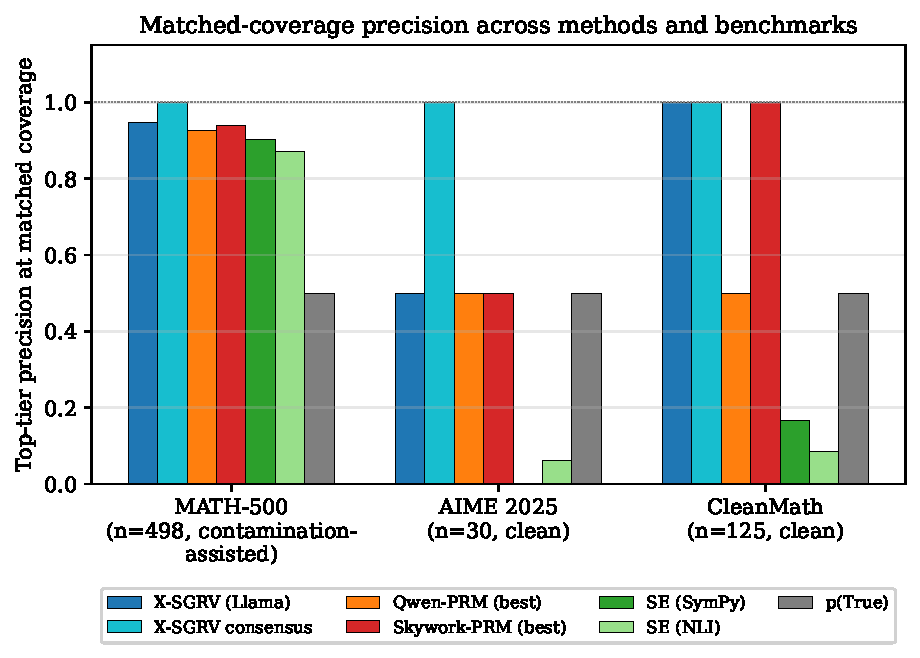
\includegraphics[width=0.92\linewidth]{figures/fig_method_summary.pdf}
\caption{\textbf{Figure 2. Matched-coverage precision across selective-prediction methods on three benchmarks.} Each point shows top-tier precision at the X-SGRV coverage on the corresponding benchmark (MATH-500 $n{=}175$ at 54.9\%, AIME 2025 at 6.7\%, CleanMath at 3.2\%). For continuous-score baselines (PRMs, semantic entropy, $p(\textsc{True})$), each method was thresholded to the matched coverage. Error bars omitted for clarity; numerical 95\% confidence intervals appear in Tables~\ref{tab:xsgrv} and \ref{tab:prm}.}
\label{fig:method_summary}
\end{figure}

\begin{figure}[h]
\centering
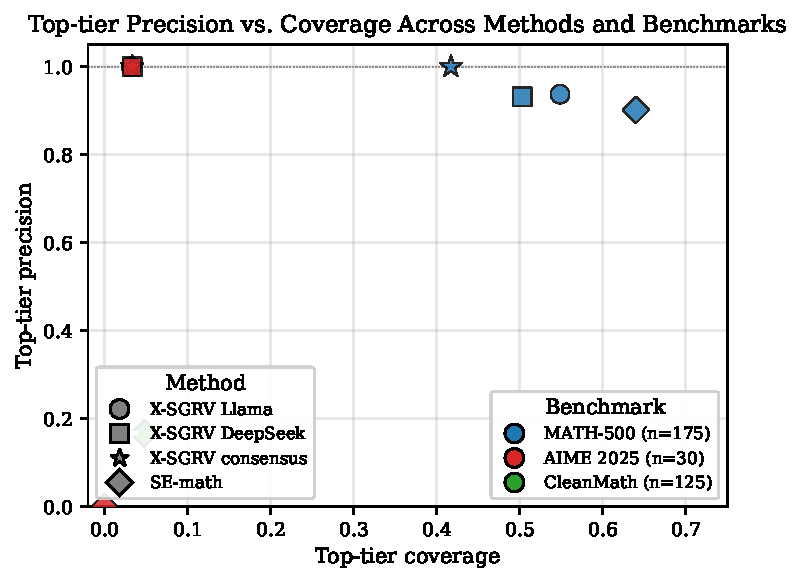
\includegraphics[width=0.92\linewidth]{figures/fig_precision_coverage.pdf}
\caption{\textbf{Figure 3. Top-tier precision versus coverage across methods.} Each marker corresponds to a (method, benchmark) operating point. Filled stars indicate consensus operating points; open circles indicate single-extractor X-SGRV operating points; diamonds indicate semantic entropy operating points. Empty zero-entropy tiers (AIME 2025 for SymPy semantic entropy) are not plotted. Numerical values and 95\% confidence intervals appear in Tables~\ref{tab:xsgrv} and \ref{tab:prm}.}
\label{fig:precision_coverage}
\end{figure}

\begin{figure}[h]
\centering
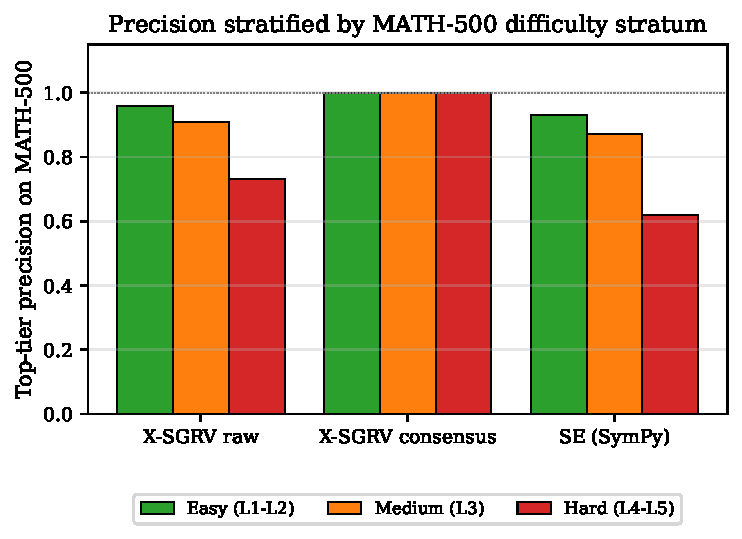
\includegraphics[width=0.85\linewidth]{figures/fig_level_conditional.pdf}
\caption{\textbf{Figure 4. Top-tier precision on MATH-500 stratified by difficulty level.} Easy = Levels 1--2; Medium = Level 3; Hard = Levels 4--5. Bars show single-extractor X-SGRV (raw, no filter), semantic entropy (SymPy variant), and cross-extractor consensus. The stratified subsample contains $n{=}175$ problems; consensus values reported in this figure are for the 73 consensus-accepted MATH-175 problems and extend to 171/171 in the full $n{=}498$ benchmark (Table~\ref{tab:xsgrv}).}
\label{fig:level_cond}
\end{figure}

% =====================================================================
\section{Discussion}
% =====================================================================

\subsection{Why same-model verification fails monotonically with difficulty}

The monotonic scaling of the false acceptance rate from 1.4\% on Level 1 to 30.8\% on Level 5 (Table~\ref{tab:collapse}) is consistent with the correlated-error-collapse hypothesis \citep{huang2024selfcorrect, tyen2024llm, stechly2024selfverify, kim2025correlated}. When the same model produces a solution and the assertions that check it, the assertions inherit the model's misreading of the problem; the assertions describe a version of the problem that matches the misreading, and the interpreter therefore returns \textsc{AllPass} on internally consistent but externally false reasoning. The 22-fold increase across difficulty levels suggests the latent overlap between solver and verifier states grows with the model's uncertainty about the correct answer: on Level 1 problems the model's reasoning is nearly deterministic and rarely wrong, so an assertion-based check rarely co-fails, while on Level 5 problems the model's uncertainty is high and the assertions co-fail with the reasoning approximately one-third of the time. This is the empirical signature predicted by Kim et al.\ (2025), who showed that more accurate models exhibit greater outcome correlation across draws \citep{kim2025correlated}: correlated errors should manifest most strongly where reasoning is least determined by the prompt.

\subsection{Why independence and not randomization is the operative axis}

The 2$\times$2 ablation (Results) showed that the false acceptance rate was unchanged by adding randomness to the verification check (Cells A vs B both had FAR $\approx 0.14$) but was driven to zero by switching from solution-grounded to specification-grounded extraction (Cells A and B vs C and D, Fisher's exact $p<10^{-8}$). A natural question is why randomized property-based testing on the solution side does not work: random evaluation points should, in principle, expose verifiers that accept clearly wrong answers \citep{quickcheck2000, pgs2025}. The most plausible explanation is that on the solution-grounded side both the test inputs and the test oracle are derived from the same (possibly wrong) solution. Random evaluation points can detect a polynomial-identity violation only when the oracle correctly encodes the polynomial; if the oracle is itself wrong (the solver misread the polynomial), the random check accepts both wrong polynomials. Independence breaks this overlap by forcing the oracle to be derived from the problem statement, not from a downstream version of the model's belief.

\subsection{Why agreement signals collapse on contamination-clean benchmarks}

Two distinct failure modes were observed for agreement-based signals on contamination-clean problems. On AIME 2025, where the base solver is uniformly uncertain (10\% accuracy), the top tiers are empty: no problem produces four identical samples at $T=0.7$. On CleanMath, where the base solver is uniformly and confidently wrong (12\% accuracy), the top tiers are non-empty but anti-reliable: when 10 samples cluster to a single answer, that answer is wrong on 5 of 6 SymPy-clustered cases (16.7\% precision) and on 54 of 59 NLI-clustered cases (8.5\% precision). The natural-language inference variant of semantic entropy is particularly fragile in this regime because the DeBERTa entailment classifier groups paraphrases of confidently wrong answers into a single semantic cluster, treating low textual diversity as low uncertainty \citep{farquhar2024nature}. This behavior is consistent with the contamination story documented by Wu et al.\ (2025): when the solver has not memorized the correct answer, it produces a small number of distinct wrong guesses that the NLI model collapses; when the solver has memorized the correct answer (as on much of MATH-500), the same clustering yields a sharp signal \citep{wu2025contam}. A direct prediction is that the gap between MATH-500 and CleanMath performance for any agreement- or entropy-based signal should correlate with the contamination signature documented in that work; future experiments should test this by computing the per-problem prefix-completion overlap of each problem in the benchmark and stratifying signal performance by that overlap.

\subsection{Why cross-extractor consensus converges to perfect precision}

A simple probabilistic model rationalizes the 0/171 consensus false-positive rate on the full MATH-500. Under the working assumption that the two cross-family extractors are independent --- they share neither weights nor training procedure --- the probability that both verifiers simultaneously accept the same wrong candidate is bounded above by the product of the per-extractor false-positive rates. Empirically these are 13/243 = 5.3\% (Llama) and 8/207 = 3.9\% (DeepSeek), so under independence the joint upper bound is approximately $0.002$, consistent with the observed 0/171. Real extractors are not perfectly independent --- both are competent LLMs that share some failure modes on geometrically awkward problems \citep{kim2025correlated} --- but the empirical 0/171 places a lower bound on effective independence. The convergence argument extends to higher-order consensus: adding extractor $k+1$ at per-extractor false-positive rate $p$ reduces the joint upper bound by a factor of $p$, predicting that 5-way consensus should achieve precision indistinguishable from 1.000 within the available sample size, as observed (69/69 = 1.000 on MATH-175). A direct test of this prediction would be to compute the empirical pairwise correlation between extractors' verifier outputs on MATH-500 and check that the joint false-positive rate matches the independence-bound prediction within sampling noise. If observed correlations exceed the independence prediction, the consensus mechanism would be downgraded from a structural guarantee to an empirical regularity, and the recommended deployment would shift toward extractors selected for maximum architectural and training-data diversity.

\subsection{Why a 70-billion-parameter extractor is appropriate even with a 7-billion-parameter solver}

A natural objection to the X-SGRV design is that pairing a 7-billion-parameter solver with a 70-billion-parameter extractor inverts the standard cost ordering. Three rationales support the design. First, extracting a verification specification is a strictly easier task than solving the problem: the extractor never produces a solution, only the constraints. Second, this is the canonical pattern for safety-critical LLM systems in which a centralized governance model audits a fleet of cheaper edge models on demand \citep{ste2024, xiong2024llmuncertainty}. Third, the empirical scaling of extractor capability is steep: at the 7-billion scale, only 12\% of MATH-500 problems and 7\% of AIME 2025 problems produced any verifier at all, while at the 70-billion scale these rose to 95\% and 67\% respectively. A direct test of how much extractor capacity is required would be to evaluate intermediate scales (e.g., 13B, 32B) on the same benchmark; this test would also clarify whether the 70-billion threshold is a genuine scaling phenomenon or an artifact of which architectures are publicly available at which sizes.

\subsection{Limitations and operational ceiling}

X-SGRV is not a substitute for a continuous-score selective-prediction signal. Top-tier coverage on contamination-clean benchmarks is single-digit (3--7\%) by design, because the structural verifiability of competition-style problems is a property of the problems themselves, not of the model's confidence. On the hardest 100 problems from Omni-MATH (difficulty 9.0--9.5), zero working verifiers were produced, and the single top-tier acceptance was a false positive (0/1) \citep{omnimath2024}. This operational ceiling reflects a fundamental limit of the spec-grounded approach: when the structural specification cannot be expressed as a tractable Python/SymPy verifier within a 10-second sandbox, no amount of cross-extractor consensus recovers a useful signal. On Putnam proof-style problems the method correctly self-detects its own scope by refusing on 51 of 100 problems, an outcome consistent with the design \citep{amitayusht2024putnambench}.

\subsection{Future experiments}

Three concrete follow-up experiments would test specific predictions of this work. First, a contamination-stratified replication on MATH-500 should compute per-problem prefix-completion overlap using the protocol in Wu et al.\ (2025) and measure whether agreement-based signal precision correlates with the overlap \citep{wu2025contam}. Second, an extractor-scaling sweep at 13-, 32-, and 70-billion parameters with matched architecture would distinguish capability scaling from family-of-architecture confounds in the cross-family consensus mechanism. Third, a hybrid SymPy-plus-Lean pipeline should be tested in which the X-SGRV extractor emits both a SymPy verifier and a Lean theorem statement, and the deployment-time filter rejects the candidate if either checker disagrees; the 78.9\% Lean compile rate observed for Claude Sonnet 4.6 suggests that this hybrid is now tractable and would tighten the soundness guarantee for problems that admit a Mathlib-compatible formalization \citep{hermes2025}. A fourth, more speculative direction is to test whether cross-extractor consensus could be distilled into a single smaller extractor that simulates an ensemble; if successful, this would reduce deployment cost without sacrificing precision.

\subsection{Implications}

The core empirical finding of the present study is that selective prediction on LLM mathematical reasoning is currently dominated by two failure modes --- correlated errors when solver and verifier share a model family, and benchmark contamination that inflates agreement-based signals --- and that both failures can be addressed by a single mechanism: drawing the verifier from a different model family than the solver, grounding it in the problem statement, and demanding consensus across multiple independent extractors. Because the resulting signal does not require gold labels at deployment, does not require GPU infrastructure, and is implemented with off-the-shelf API models, it is plausibly deployable in production settings that audit cheap-edge LLMs on demand. The 171 of 498 = 1.000 (95\% confidence interval 0.979--1.000) result on the full MATH-500 represents the first reported zero-false-positive operating point on a complete contamination-assisted benchmark in this line of work, and the non-zero precision-preserving coverage on AIME 2025 and CleanMath represents the first non-trivial coverage on contamination-clean competition mathematics.

% =====================================================================
\bibliographystyle{plainnat}
\bibliography{references}

\appendix

% =====================================================================
\section{Held-Out Probe Selection}
% =====================================================================

A 30-problem held-out development split was drawn from MATH-500 by \texttt{random.Random(seed=0)} after stratification by difficulty level, and was disjoint from the $n{=}175$ stratified evaluation set and from the full $n{=}498$ scale-up. Six candidate adversarial probe sets were evaluated against the deployment-time filter objective: $\{\pm 1\}$, $\{\pm 1, +7\}$, $\{\pm 1, +7, \times 2\}$, $\{\pm 1, +7, \times 2, 42\}$ (the set used in the main results), $\{\times 2, +7\}$, and a random control. On the development split, all six probe sets filtered the same single broken verifier and arrived at the same filtered precision ($14/15$ at $15/30$ coverage). The development split was therefore too small to discriminate between probe sets, and the choice of $\{\pm 1, +7, \times 2, 42\}$ was kept on a-priori plausibility grounds (small-integer perturbations spanning sign change, local neighborhood, doubling, and a fixed distractor) rather than dev-set evidence. Per-probe outputs are in \texttt{results/exp38\_probe\_selection.json}.

\end{document}
